En esta secci\'on, presentaremos los resultados obtenidos en los experimentos utilizando lo definido en la secci\'on de desarrollo.

\subsection{Red hogareña}

\subsubsection{Fuente Unicast-Multicast}

\hspace*{-1.5cm}
 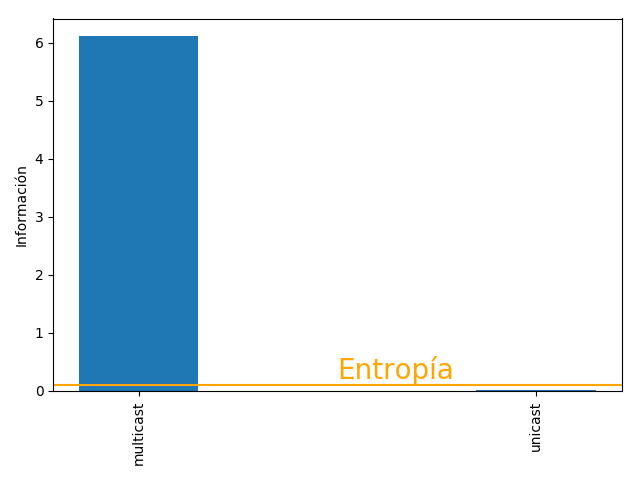
\includegraphics[scale=0.6]{../plots/mauro_s1_informacion.png}
 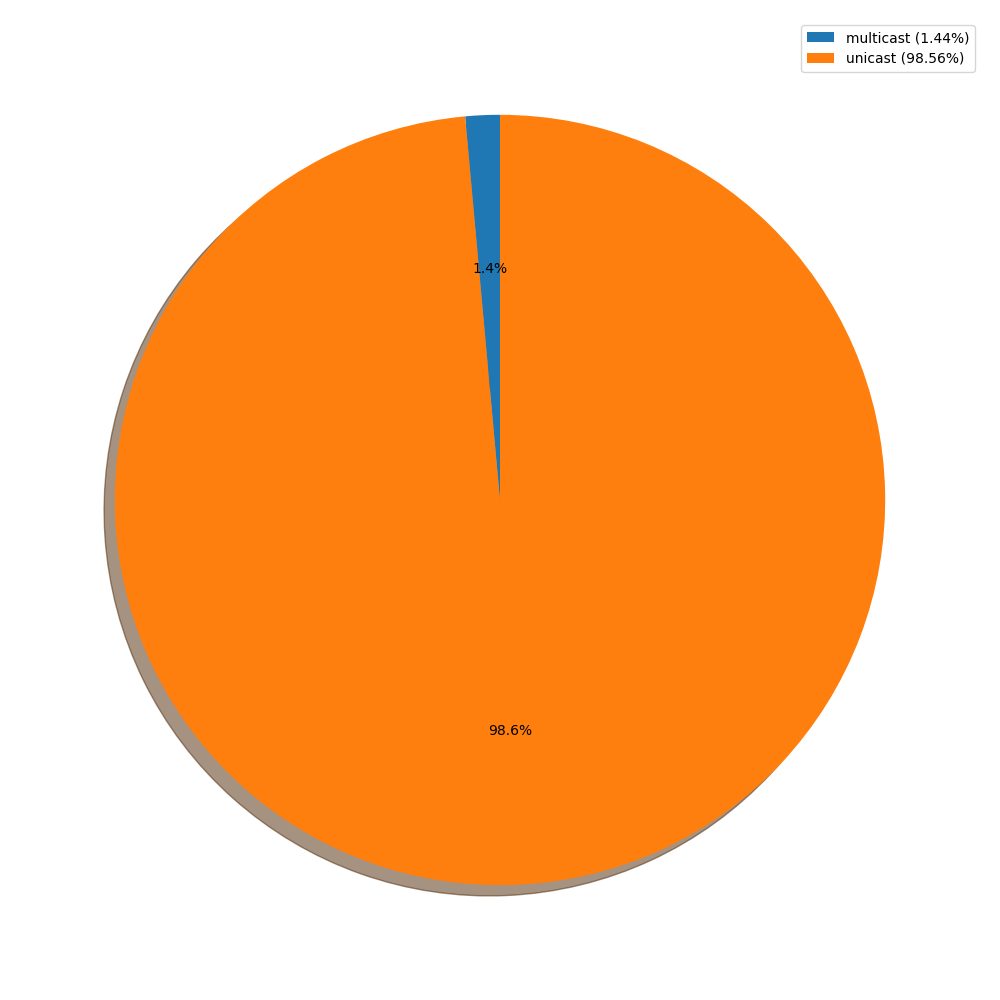
\includegraphics[scale=0.4]{../plots/mauro_s1_probabilidades.png}

Como podemos ver 
\subsubsection{Fuente ARP}

\hspace*{-1.5cm}
 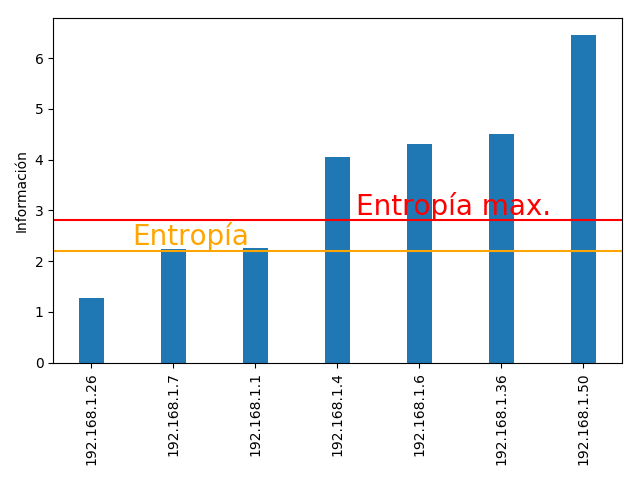
\includegraphics[scale=0.6]{../plots/mauro_s2_informacion.png}
 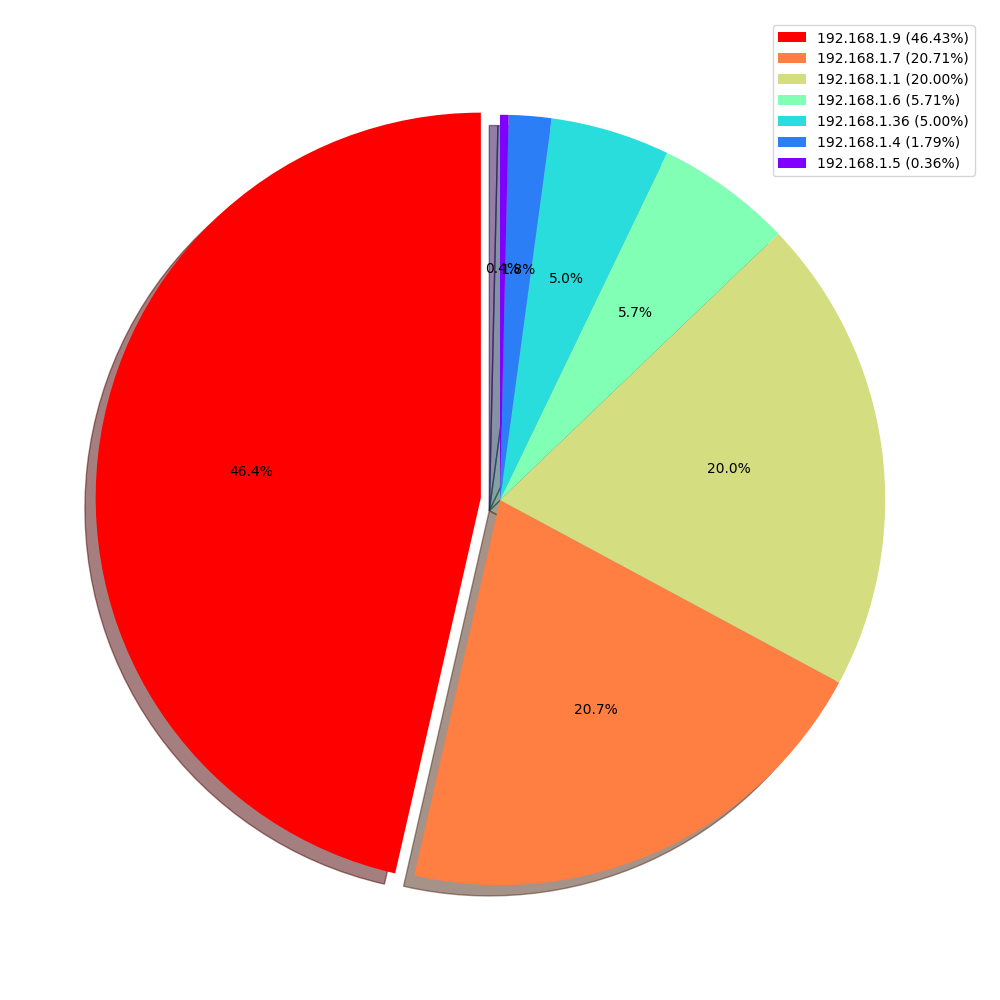
\includegraphics[scale=0.4]{../plots/mauro_s2_probabilidades.png}

\subsubsection{Topolog\'ia de la Red}
\begin{center}
 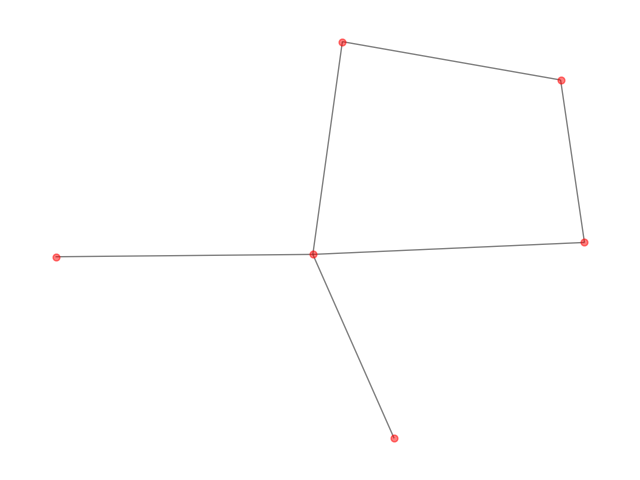
\includegraphics[scale=0.6]{../plots/mauro_s2_topologia.png}
\end{center}

\subsection{Experimento Chino}

\subsubsection{Fuente Unicast-Multicast}

\hspace*{-1.5cm}
 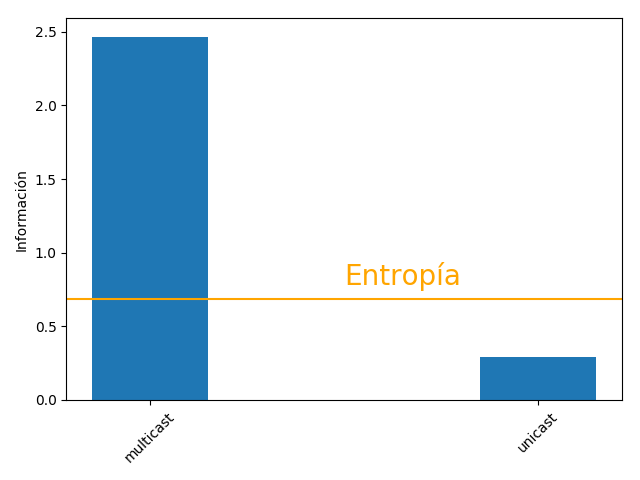
\includegraphics[scale=0.6]{../plots/trabajo_s1_informacion.png}
 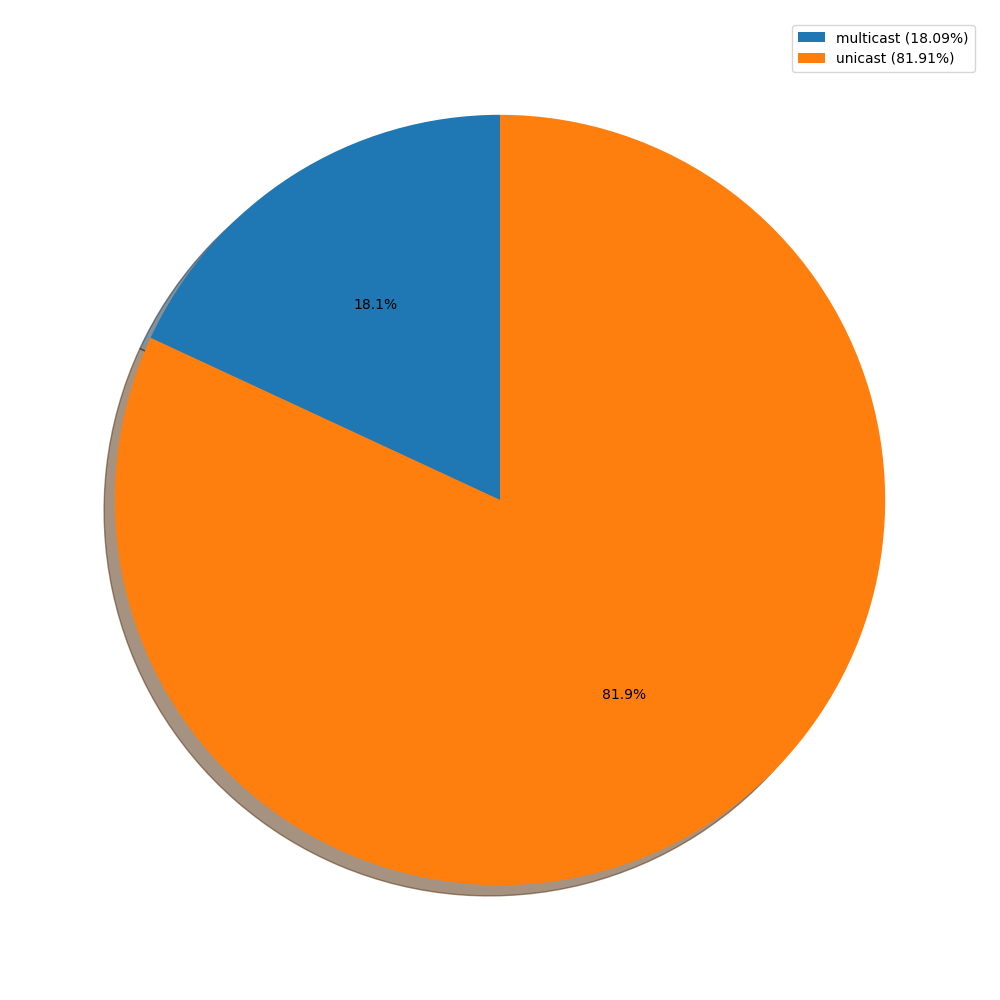
\includegraphics[scale=0.4]{../plots/trabajo_s1_probabilidades.png}

\subsubsection{Fuente ARP}

\hspace*{-1.5cm}
 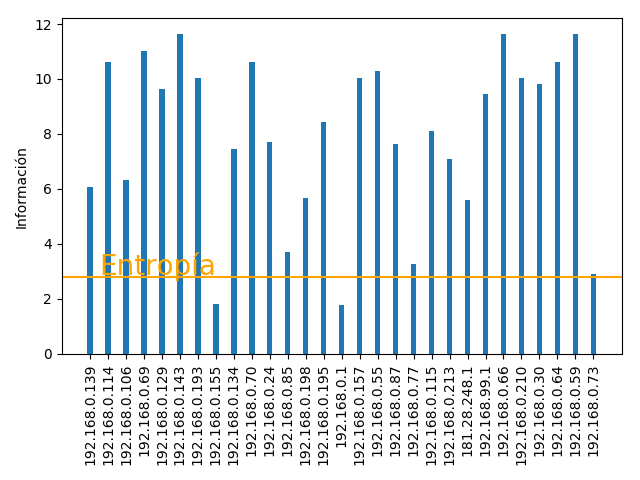
\includegraphics[scale=0.6]{../plots/trabajo_s2_informacion.png}
 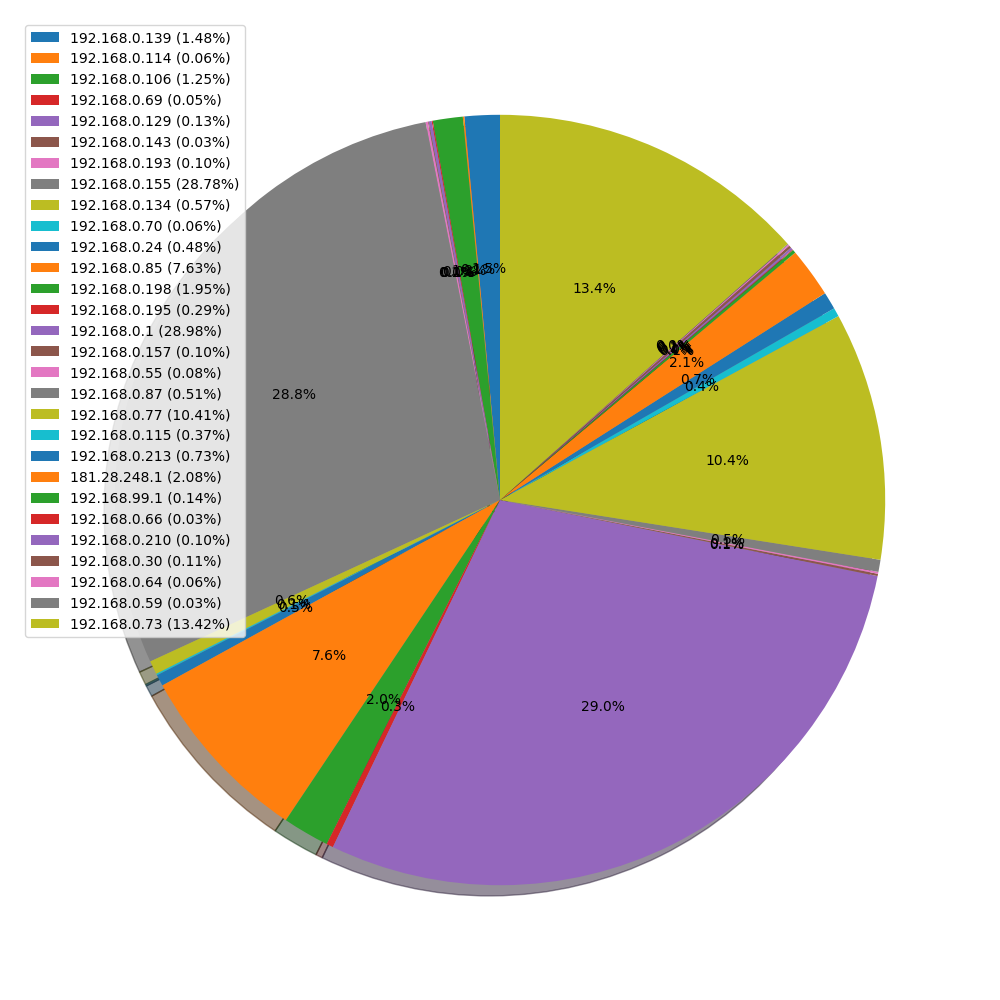
\includegraphics[scale=0.4]{../plots/trabajo_s2_probabilidades.png}


\subsubsection{Topolog\'ia de la Red}
\begin{center}
 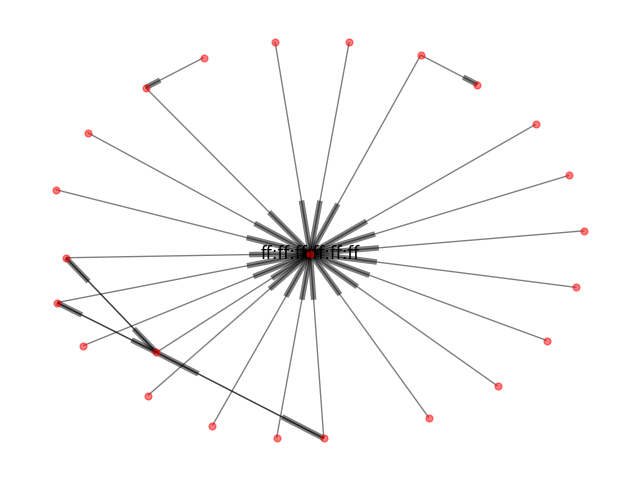
\includegraphics[scale=0.6]{../plots/trabajo_s2_topologia.png}
\end{center}

\subsection{Experimento Tavo}

Arreglar cosas